% !TeX root = ../main.tex

\chapter{Verwandte Arbeiten}\label{chapter:background}
	
	%In this chapter, \dots

	%\section{Math} \label{sec:full_grids}
	
		%Math:
		%\begin{align}
			%\Phi(x) = \max(1 - \abs{x}, 0)
		%\end{align}
		
	 %\subsection{Example Figure} \label{sec:back_nodal_hierarchical_basis}
		
		%\begin{figure}[htbp]
			%\centering
			%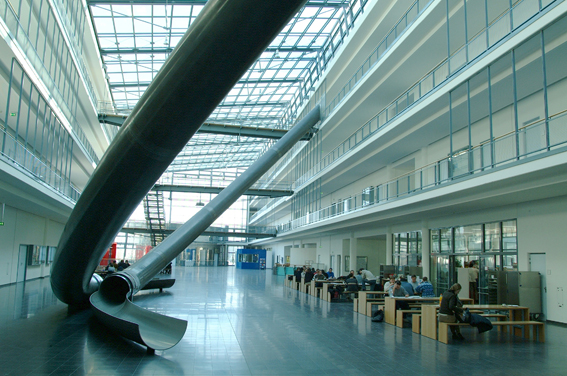
\includegraphics[width=0.5\textwidth]{figures/tum.jpg}
			%\caption{Example picture that was taken from an external source \takenFrom{asc_notes}.}
			%\label{fig:nodalBasis}
		%\end{figure}
		
		%References on figures work like this: blblablabla (see \refFigure{fig:nodalBasis}). If you used external knowledge for a paragraph, use the cite command at the very end of a sentence but right before the full stop \cite{ba_molzer}.
		
		%If you use an $l$ for math symbols, use $\ell$ instead for better readability.
		
	Vor dem Behandeln eines Problems ist es wichtig sich ebenso darüber zu informieren, was in diesem Bereich bereits in anderen Arbeiten behandelt wurde und welche Ergebnisse dabei erzielt wurden.
	\todo{Schönerer Einstieg!}
	Die Forschungen im Bereich der Platzierung und des Designs von Benutzeroberflächen in Desktop-Anwendungen \todo{Formulieren} Jahrelange Erfahrung
	
	
	Auch mit der Platzierung in virtuellen 3D-Umgebungen haben sich einige Leute beschäftigt. \todo{Beispiele und schöner}
	Zu dem Thema plattformübergreifender Programme in der erweiterten Realität gibt es ebenso schon einige Ansätze \todo{Links}, aber bei näherer Betrachtung dieser Programme fällt auf, dass hierbei häufig auf graphische Benutzeroberflächen weitestgehend verzichtet wurde. 
	- eventuell Verknüpfung zu diegetic?
		
	\section{Priorisieren von Benutzeroberflächen}
		\todo{Abschnitt überprüfen und Beweise einfügen}
		Das Umstrukturieren von Menüs ist nicht trivial, denn jede Veränderung in der Benutzeroberfläche kann das Nutzererlebnis drastisch verändern, falls der Nutzer dadurch irritiert wird. Dies ist sowohl in zweidimensionalen Programmen der Fall, wie auch in der virtuellen dreidimensionalen Welt. Mit diesem Nutzererlebnis setzt sich seit einigen Jahren der Bereich des UX Designs\todo{UX erklären} auseinander. 
		- nicht zu viel und nicht wenig Info
		Es gibt dabei allerdings keine perfekte Lösung, da es sich dabei um ein subjektives Erlebnis handelt\todo{Link zu UX 1}.
		Um aber das Risiko einer Verschlechterung des Nutzungserlebnisses gering zu halten, hilft es die vorhandenen Informationen zu priorisieren und abhängig davon zu entscheiden, wann und wie diese dem Nutzer angezeigt werden. Dazu kann man zum Beispiel Untermenüs oder Popups \todo{Anderes Wort!} verwenden.
		
		- UX
		- Prioritätsgruppen
		- Umsetzung in 2D
		
	\section{Positionierung in 2D}
		Das verbreitetste Konzept zur Umsetzung von ... ist das WIMP-Konzept...
		- gewöhnlich Fenstergebunden WIMP
		- Windows Icons Menus Pointers
		Die Abkürzung steht für Windows, Icons, Menus, Pointers und beschreibt somit bereits wie Informationen und Funktionen dargestellt werden.
		\todo{Referenz WIMP}
		- Menüs / Fenster
		Menüs geben eine Auswahl von Funktionen in Form von ...
		- Bildschirmränder
		
		
	\section{Positionierung in 3D (VR/AR auch ohne)}
		- 3D Programm: UI in Welt platziert
		- Üblich Hände und Kopf oder an statischen Objekten
		- Beispiele! Zylinderbild
		
		\begin{figure}[htbp]
			\centering
			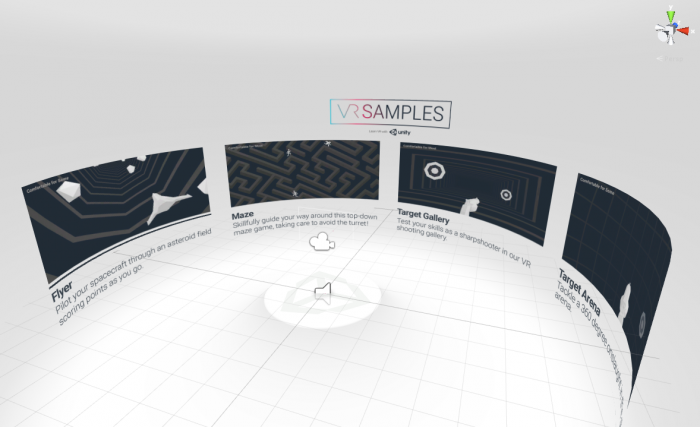
\includegraphics[width=0.75\textwidth]{figures/cylinder_mapping.png}
			\caption{Example picture that was taken from an external source \takenFrom{asc_notes}.}
			\label{fig:cylinder_mapping}
		\end{figure}
		- dreidimensionale Benutzeroberflächen